%%
%% This is file `./samples/shortsample.tex',
%% generated with the docstrip utility.
%%
%% The original source files were:
%%
%% apa6.dtx  (with options: `shortsample')
%% ----------------------------------------------------------------------
%% 
%% apa6 - A LaTeX class for formatting documents in compliance with the
%% American Psychological Association's Publication Manual, 6th edition
%% 
%% Copyright (C) 2011-2017 by Brian D. Beitzel <brian at beitzel.com>
%% 
%% This work may be distributed and/or modified under the
%% conditions of the LaTeX Project Public License (LPPL), either
%% version 1.3c of this license or (at your option) any later
%% version.  The latest version of this license is in the file:
%% 
%% http://www.latex-project.org/lppl.txt
%% 
%% Users may freely modify these files without permission, as long as the
%% copyright line and this statement are maintained intact.
%% 
%% This work is not endorsed by, affiliated with, or probably even known
%% by, the American Psychological Association.
%% 
%% ----------------------------------------------------------------------
%% 
\documentclass[jou]{apa6}

\usepackage[american]{babel}

\usepackage{csquotes}
\usepackage[style=apa,sortcites=true,sorting=nyt,backend=biber]{biblatex}
\DeclareLanguageMapping{american}{american-apa}
\addbibresource{bibliography.bib}


%%%%%%%%%%%%%%%%%%%%%%%%%%%%%%%%%%%%%%%%
%% Discrete Structures
%% The start of RBS stuff
%%%%%%%%%%%%%%%%%%%%%%%%%%%%%%%%%%%%%%%%

% Working internal and external links in PDF
\usepackage{hyperref}
% Extra math symbols in LaTeX
\usepackage{amsmath}
\usepackage{gensymb}
\usepackage{amssymb}
% Enumerations with (a), (b), etc.
\usepackage{enumerate}

\let\OLDitemize\itemize
\renewcommand\itemize{\OLDitemize\addtolength{\itemsep}{-6pt}}

\usepackage{etoolbox}
\makeatletter
\preto{\@verbatim}{\topsep=3pt \partopsep=3pt }
\makeatother

% These sizes redefine APA for A4 paper size
\oddsidemargin 0.0in
\evensidemargin 0.0in
\textwidth 6.27in
\headheight 1.0in
\topmargin -24pt
\headheight 12pt
\headsep 12pt
\textheight 9.19in



\title{Quiz for Week02}
\author{Discrete Structures, Fall 2020}
\affiliation{RBS}

\leftheader{Discrete Structures (W2): Quiz}

\abstract{%
}

%\keywords{}

\begin{document}
%\maketitle

\twocolumn
{\Large Discrete Structures (W3): Quiz}

\thispagestyle{empty}

\vspace{6pt}
{\bf Question 1.} We have the following
truth table ("0" means False, "1" means "True"). 
Find the correct DNF (Disjunctive Normal Form). 
(Multiple answers may be true, since
there may more than one way to write DNFs for the same Boolean 
function.)


\begin{center}
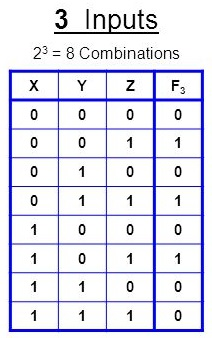
\includegraphics[width=2in]{quiz3/table2.jpg}
\end{center}


{\large
\noindent
{\normalsize \bf (A)}
$$(X \wedge \neg Y \wedge Z) \vee (\neg X \wedge Y \wedge Z)$$
{\normalsize \bf (B)} % Fine
$$(\neg Z \wedge Y \wedge Z) \vee (\neg Y \wedge Z)$$
{\normalsize \bf (C)} % Fine
$$(\neg X \wedge Z) \vee (X \wedge \neg Y \wedge Z)$$
{\normalsize \bf (D)}
$$(\neg X \wedge \neg Y \wedge Z) \vee (\neg X \wedge Y)$$
}



{\bf Question 2.} Identify, which is the correct CNF (Conjunctive Normal Form) that computes the same thing as 
Peirce's arrow: $a \downarrow b = \neg (a \vee b)$.
(Multiple answers may be true, since
there may more than one way to write CNFs for the same Boolean 
function.)

{\large
\noindent
{\normalsize \bf (A)} %% Fine
$$(\neg a \vee \neg b) \wedge (\neg a \vee b) \wedge (a \vee \neg b)$$
{\normalsize \bf (B)}
$$(a \vee b) \wedge (\neg a \vee b) \wedge (a \vee \neg b)$$
{\normalsize \bf (C)}
$$\neg a \vee \neg b$$
{\normalsize \bf (D)} %% Fine
$$\neg a \wedge (a \vee \neg b)$$
}



{\bf Question 3.} We have predicates $A(p,i,r)$ (a Python program 
$p \in \mathcal{P}$ receives input $i \in \mathbb{Z}^{+}$ and answers
with the result $r \in \mathbb{Z}^{+}$); $H(p,i)$ (program $p$ halts on input $i$), 
and $C(i,r)$ (the correct/expected output for input $i$ is $r$). 
Identify the predicate expression that expresses the following English sentence:\\
``For all inputs that are sufficiently large, the given program $p$ 
halts and produces outputs that are correct; for some (finitely many) inputs $p$ 
may loop forever, but it is never incorrect.''

{\large
\noindent
{\normalsize \bf (A)}
$$\forall p \in \mathcal{P}\; \forall i \in \mathbb{Z}^{+}\; \forall r \in \mathbb{Z}^{+},$$
$$((i > M \,\wedge\, H(p,i)) \vee (A(p,i,r) \wedge C(i,r)))$$
{\normalsize \bf (B)}
$$\exists M \in \mathbb{Z}^{+}\; \forall i \in \mathbb{Z}^{+}\;
\forall r \in \mathbb{Z}^{+},$$
$$((i < M \,\wedge\, \neg H(p,i)) \vee (A(p,i,r) \wedge C(i,r)))$$\\
{\normalsize \bf (C)}
$$\forall p \in \mathcal{P}\; M \in \mathbb{Z}^{+}\; \forall i \in \mathbb{Z}^{+}\;
\forall r \in \mathbb{Z}^{+},$$
$$((i > M \,\wedge\, H(p,i)) \vee (A(p,i,r) \wedge C(i,r)))$$
{\normalsize \bf (D)}
$$\forall p \in \mathcal{P}\; \forall i \in \mathbb{Z}^{+}\;
\forall r \in \mathbb{Z}^{+},$$ 
$$((i > M \,\wedge\, H(p,i)) \vee (A(p,i,r) \wedge C(i,r)))$$
}



{\bf Question 4.} For the quantifiers 
($A(p,i,r)$, $H(p,i)$, $C(i,r)$) defined in the previous question, 
the following expression is given:
$$\forall p \in \mathcal{P} 
\exists i \in \mathbb{Z}^{+}\; \exists j \in \mathbb{Z}^{+},$$
$$(j > i \,\wedge\, (H(p,i) \rightarrow H(p,j)).$$
Which sentence is expressed by this?

{\bf (A)} Each Python program halts for at least 2 inputs.\\ 
{\bf (B)} Each Python program halts for infinitely many inputs. \\
{\bf (C)} There is no Python program that halts on exactly 1 input. \\
{\bf (D)} For each Pyton program there is the largest input for which it halts.


{\bf Question 5.} 
There is a set of 2 students $S = \{ s_1, s_2 \}$ and 
a set of 5 chairs $C = \{ c_1, c_2, c_3, c_4, c_5 \}$. 
Find, how many such functions $f\,:\,S \rightarrow C$ exist (a function 
by definition is a mapping that assigns a chair for each student;
it is NOT always true that different students get different chairs
or that all chairs are occupied). Please find the total number of 
such functions, also the number of injective, surjective
and bijective functions among them.

Your answer should be a comma-separated list of 4 numbers
(e.g. 10,11,12,13 means that 10 is the total, 11 - injective, 12 - surjective, 13 - bijective).





{\bf Question 6.} 
Predicate S(x,y,z) is true iff x*y=z.
Given the following equation:
{\large
$$\forall u \in \mathbb{Z}^{+}\;\forall v \in \mathbb{Z}^{+}\;
\forall p \in \mathbb{Z}^{+}\;\forall q \in \mathbb{Z}^{+}\;
\exists k \in \mathbb{Z}^{+},$$
$$S(x,u,y) \wedge S(x,v,z) \wedge
S(d,p,y) \wedge S(d,q,z)$$
$$\rightarrow S(d,k,x).$$
}

Which statement is expressed by this expression?\\
{\bf (A)} $d$ is the greatest common divisor of $y$ and $z$,\\
{\bf (B)} $x$ is the greatest common divisor of $p$ and $q$,\\
{\bf (C)} $x$ is the greatest common divisor of $y$ and $z$,\\
{\bf (D)} $d$ is the greatest common divisor of $u$ and $v$.


{\bf Question 7.} 
\begin{center}
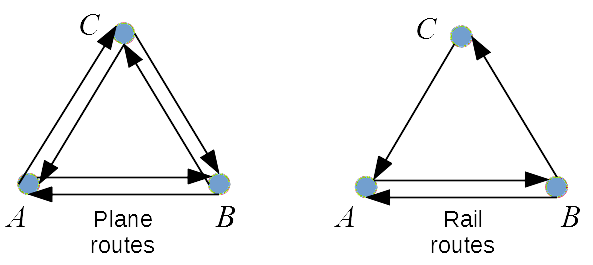
\includegraphics[width=2in]{relation-graphs.png}
\end{center}

Find the predicate expression that expresses this statement: 
"For the two given cities 'x' and 'y' there is a two-leg trip
using planes, but there is no two-leg trip using rail."
(We call a trip "two-leg", if it uses exactly two plane flights
or exactly two rail links.)

\begin{verbatim}
(A) forall x y z: City,  Plane(x,z) /\ Plane(z,x) /\ ~(Rail(x,z) /\ Rail(z,y))

(B) exists z: City, Plane(x,z) /\ Plane(z,x) /\ ~(Rail(x,z) /\ Rail(z,y))
	
(C) forall x y: City, exists z: City, Plane(x,z) /\ Plane(z,x) /\  (~Rail(x,z) \/ ~Rail(z,y))
	
(D) exists z1: City, forall z2: City, Plane(x,z1) /\ Plane(z1,x) /\ (~Rail(x,z2) \/ ~Rail(z2,y))
\end{verbatim}



\end{document}
